%!TEX TS-program = xelatex
\documentclass[12pt,a4paper, oneside]{extreport}

%%%%%%%%%% Програмный код %%%%%%%%%%
% \usepackage{minted}
% Включает подсветку команд в программах!
% Нужно, чтобы на компе стоял питон, надо поставить пакет Pygments, в котором он сделан, через pip.

% Для Windows: Жмём win+r, вводим cmd, жмём enter. Открывается консоль.
% Прописываем pip install Pygments
% Заходим в настройки texmaker и там прописываем в PdfLatex или XelaTeX:
% pdflatex -shell-escape -synctex=1 -interaction=nonstopmode %.tex

% Для Linux: Открываем консоль. Убеждаемся, что у вас установлен pip командой pip --version
% Если он не установлен, ставим его: sudo apt-get install python-pip
% Ставим пакет sudo pip install Pygments

% Для Mac: Всё то же самое, что на Linux, но через brew.

% После всего этого вы должны почувствовать себя тру-программистами!
% Документация по пакету хорошая. Сам читал, погуглите!

%%%%%%%%%% Математика %%%%%%%%%%
\usepackage{amsmath,amsfonts,amssymb,amsthm,mathtools}
% Показывать номера только у тех формул, на которые есть \eqref{} в тексте.
%\mathtoolsset{showonlyrefs=true}
%\usepackage{leqno} % Нумерация формул слева
%\usepackage{tipa} %Для формулки из логитов


\usepackage{hyphenat}


%%%%%%%%%% Шрифты %%%%%%%%
\usepackage[english, russian]{babel} % выбор языка для документа
\usepackage[utf8]{inputenc} % задание utf8 кодировки исходного tex файла
\usepackage[X2,T2A]{fontenc}        % кодировка

\usepackage{fontspec}         % пакет для подгрузки шрифтов
\setmainfont{Times New Roman}       % задаёт основной шрифт документа

\usepackage{unicode-math}      % пакет для установки математического шрифта
\setmathfont{Asana-Math.otf}    % шрифт для математики

% Конкретный символ из конкретного шрифта
% \setmathfont[range=\int]{Neo Euler}


%%%%%%%%%% Работа с картинками %%%%%%%%%
\usepackage{graphicx}                  % Для вставки рисунков
\usepackage{graphics}
\graphicspath{{images/}{pictures/}}    % можно указать папки с картинками
\usepackage{wrapfig}                   % Обтекание рисунков и таблиц текстом


%%%%%%%%%% Работа с таблицами %%%%%%%%%%
\usepackage{tabularx}            % новые типы колонок
\usepackage{tabulary}            % и ещё новые типы колонок
\usepackage{array,delarray}      % Дополнительная работа с таблицами
\usepackage{longtable}           % Длинные таблицы
\usepackage{multirow}            % Слияние строк в таблице
\usepackage{float}               % возможность позиционировать объекты в нужном месте

\usepackage{booktabs}            % таблицы как в книгах
% Заповеди из документации к booktabs:
% 1. Будь проще! Глазам должно быть комфортно
% 2. Не используйте вертикальные линни
% 3. Не используйте двойные линии. Как правило, достаточно трёх горизонтальных линий
% 4. Единицы измерения - в шапку таблицы
% 5. Не сокращайте .1 вместо 0.1
% 6. Повторяющееся значение повторяйте, а не говорите "то же"
% 7. Есть сомнения? Выравнивай по левому краю!

%  вычисляемые колонки по tabularx
\newcolumntype{C}{>{\centering\arraybackslash}X}
\newcolumntype{L}{>{\raggedright\arraybackslash}X}
\newcolumntype{Y}{>{\arraybackslash}X}
\newcolumntype{Z}{>{\centering\arraybackslash}X}


%%%%%%%%%% Графика и рисование %%%%%%%%%%
\usepackage{tikz, pgfplots}      % язык для рисования графики из latex'a

%%%%%%%%%% Гиперссылки %%%%%%%%%%
\usepackage{xcolor}              % разные цвета

\usepackage{hyperref}
\hypersetup{
	unicode=true,           % позволяет использовать юникодные символы
	colorlinks=true,       	% true - цветные ссылки, false - ссылки в рамках
	urlcolor =blue,         % цвет ссылки на url
	linkcolor=black,        % внутренние ссылки
	citecolor=black,        % на библиографию
	breaklinks              % если ссылка не умещается в одну строку, разбивать ли ее на две части?
}


%%%%%%%%%% Другие приятные пакеты %%%%%%%%%
\usepackage{multicol}       % несколько колонок
\usepackage{verbatim}       % для многострочных комментариев
\usepackage{cmap} % для кодировки шрифтов в pdf

\usepackage{enumitem} % дополнительные плюшки для списков
%  например \begin{enumerate}[resume] позволяет продолжить нумерацию в новом списке

\usepackage{todonotes} % для вставки в документ заметок о том, что  осталось сделать
% \todo{Здесь надо коэффициенты исправить}
% \missingfigure{Здесь будет Последний день Помпеи}
% \listoftodos --- печатает все поставленные \todo'шки



%%%%%%%%%%%%%% ГОСТОВСКИЕ ПРИБАМБАСЫ %%%%%%%%%%%%%%%

%%% размер листа бумаги
\usepackage[paper=a4paper,top=15mm, bottom=15mm,left=35mm,right=10mm,includehead]{geometry}


\usepackage{setspace}
\setstretch{1.33}     % Межстрочный интервал
\setlength{\parindent}{1.5em} % Красная строка.


%\flushbottom       % Эта команда заставляет LaTeX чуть растягивать строки, чтобы получить идеально прямоугольную страницу
\righthyphenmin=2  % Разрешение переноса двух и более символов
\widowpenalty=10000  % Наказание за вдовствующую строку (одна строка абзаца на этой странице, остальное --- на следующей)
%\clubpenalty=10000  % Наказание за сиротствующую строку (омерзительно висящая одинокая строка в начале страницы)
\tolerance=1000     % Ещё какое-то наказание.


% Нумерация страниц сверху по центру
\usepackage{fancyhdr}
\pagestyle{fancy}
\fancyhead{ } % clear all fields
\fancyfoot{ } % clear all fields
\fancyhead[C]{\thepage}
% Чтобы не прорисовывалась черта!
\renewcommand{\headrulewidth}{0pt}


% Нумерация страниц с надписью "Глава"
\usepackage{etoolbox}
\patchcmd{\chapter}{\thispagestyle{plain}}{\thispagestyle{fancy}}{}{}


%%% Заголовки
\usepackage[indentfirst]{titlesec}{\raggedleft}
% Заголовки по левому краю
% опция identfirst устанавливает отступ в первом абзаце



% В Linux этот пакет сделан косячно. Исправляет это следующий непонятный кусок кода.
\makeatletter
\patchcmd{\ttlh@hang}{\parindent\z@}{\parindent\z@\leavevmode}{}{}
\patchcmd{\ttlh@hang}{\noindent}{}{}{}
\makeatother


% Редактирования Глав и названий
\titleformat{\chapter}
{\normalfont\large\bfseries}
{\thechapter }{0.5 em}{}

% Редактирование ненумеруемых глав chapter* (Введение и тп)
\titleformat{name=\chapter,numberless}
{\centering\normalfont\bfseries\large}{}{0.25em}{\normalfont}

% Убирает чеканутые отступы вверху страницы
\titlespacing{\chapter}{0pt}{-\baselineskip}{\baselineskip}

% Более низкие уровни
\titleformat{\section}{\bfseries}{\thesection}{0.5 em}{}
\titleformat{\subsection}{\bfseries}{\thesubsection}{0.5 em}{}

\titlespacing*{\section}{0 pt}{\baselineskip}{\baselineskip}
\titlespacing*{\subsection}{0 pt}{\baselineskip}{\baselineskip}


% Содержание. Команды ниже изменяют отступы и рисуют точечки!
\usepackage{titletoc}

\titlecontents{chapter}
[1em] %
{\normalsize}
{\contentslabel{1 em}}
{\hspace{-1 em}}
{\normalsize\titlerule*[10pt]{.}\contentspage}

\titlecontents{section}
[3 em] %
{\normalsize}
{\contentslabel{1.75 em}}
{\hspace{-1.75 em}}
{\normalsize\titlerule*[10pt]{.}\contentspage}

\titlecontents{subsection}
[6 em] %
{\normalsize}
{\contentslabel{3 em}}
{\hspace{-3 em}}
{\normalsize\titlerule*[10pt]{.}\contentspage}


% Правильные подписи под таблицей и рисунком
% Документация к пакету на русском языке!
\usepackage[tableposition=top, singlelinecheck=false]{caption}
\usepackage{subcaption}


\DeclareCaptionStyle{base}%
[justification=centering,indention=0pt]{}
\DeclareCaptionLabelFormat{gostfigure}{Рисунок #2}
\DeclareCaptionLabelFormat{gosttable}{Таблица #2}

\DeclareCaptionLabelSeparator{gost}{~---~}
\captionsetup{labelsep=gost}

\DeclareCaptionStyle{fig01}%
[margin=5mm,justification=centering]%
{margin={3em,3em}}
\captionsetup*[figure]{style=fig01,labelsep=gost,labelformat=gostfigure,format=hang}

\DeclareCaptionStyle{tab01}%
[margin=5mm,justification=centering]%
{margin={3em,3em}}
\captionsetup*[table]{style=tab01,labelsep=gost,labelformat=gosttable,format=hang}


% межстрочный отступ в таблице
\renewcommand{\arraystretch}{1.2}



% многостраничные таблицы под РОССИЙСКИЙ СТАНДАРТ
% ВНИМАНИЕ! Обязательно за CAPTION !
\usepackage{fr-longtable}



%Более гибкие спсики
\usepackage{enumitem}
% сообщаем окружению о том, что существует такая штук как нумерация русскими буквами.
\makeatletter
\AddEnumerateCounter{\asbuk}{\russian@alph}{щ}
\makeatother


%%% ГОСТОВСКИЕ СПИСКИ

% Первый тип списков. Большая буква.
\newlist{Enumerate}{enumerate}{1}

\setlist[Enumerate,1]{labelsep=0.5em,leftmargin=1.25em,labelwidth=1.25em,
	parsep=0em,itemsep=0em,topsep=0ex, before={\parskip=-1em},label=\arabic{Enumeratei}.}


% Второй тип списков. Маленькая буква.
\setlist[enumerate]{label=\arabic{enumi}),parsep=0em,itemsep=0em,topsep=0.75ex, before={\parskip=-1em}}


% Третий тип списков. Два уровня.
\newlist{twoenumerate}{enumerate}{2}
\setlist[twoenumerate,1]{itemsep=0mm,parsep=0em,topsep=0.75ex,, before={\parskip=-1em},label=\asbuk{twoenumeratei})}
\setlist[twoenumerate,2]{leftmargin=1.3em,itemsep=0mm,parsep=0em,topsep=0ex, before={\parskip=-1em},label=\arabic{twoenumerateii})}


% Четвёртый тип списков. Список с тире.
\setlist[itemize]{label=--,parsep=0em,itemsep=0em,topsep=0ex, before={\parskip=-1em},after={\parskip=-1em}}


%%% WARNING WARNING WARNIN!
%%% Если в списке предложения, то должна по госту стоять точка после цифры => команда Enumerate! Если идет перечень маленьких фактов, не обособляемых предложений то после цифры идет скобка ")" => команда enumerate! Если перечень при этом ещё и двууровневый, то twoenumerate.




%%%%%%%%%% Список литературы %%%%%%%%%%

%\usepackage[%
%backend=biber, %подключение пакета biber (тоже нужен)
%bibstyle=gost-numeric, %подключение одного из четырех главных стилей biblatex-gost
%sorting=ntvy, %тип сортировки в библиографии
%]{biblatex}
\usepackage[backend=biber,style=gost-numeric, maxbibnames=9,maxcitenames=2,uniquelist=false, babel=other]{biblatex}

% Справка по 4 главным стилям для ленивых:
% gost-inline  ссылки внутри теста в круглых скобках
% gost-footnote подстрочные ссылки
% gost-numeric затекстовые ссылки
% gost-authoryear тоже затекстовые ссылки, но немного другие

% Подробнее смотри страницу 4 документации. Она на русском.

% Ещё немного настроек
\DeclareFieldFormat{postnote}{#1} %убирает с. и p.
\renewcommand*{\mkgostheading}[1]{#1} % только лишь убираем курсив с авторов


\addbibresource{diploma.bib} % сюда нужно вписать свой bib-файлик.

% Этот кусок кода выносит русские источники на первое место. Костыль описали авторы пакета в руководстве к нему. Подробнее смотри:
% https://github.com/odomanov/biblatex-gost/wiki/Как-сделать%2C-чтобы-русскоязычные-источники-предшествовали-остальным
\DeclareSourcemap{
	\maps[datatype=bibtex]{
		\map{
			\step[fieldsource=langid, match=russian, final]
			\step[fieldset=presort, fieldvalue={a}]
		}
		\map{
			\step[fieldsource=langid, notmatch=russian, final]
			\step[fieldset=presort, fieldvalue={z}]
		}
	}
}

\DefineBibliographyStrings{english}{%
	pages = {P\adddot},
	number = {№},
}


\begin{document} % Начала документа

\thispagestyle{empty} % Чтобы избежать нумерации титульника

% Если для какой-то страницы хочется сделать своё уникальное оформление, как например для титульника или списка литературы, то можно использовать окружение \begingroup ... \endgroup. 
\begingroup
\setstretch{1}   % Убираем полторашные интервалы на титульнике
\begin{center}
\small \bfseries Федеральное государственное бюджетное образовательное учреждение высшего образования

<<РОССИЙСКАЯ АКАДЕМИЯ НАРОДНОГО ХОЗЯЙСТВА и\\ ГОСУДАРСТВЕННОЙ СЛУЖБЫ \\
при Президенте Российской Федерации>>

\vspace{2ex}

\bfseries
ЭКОНОМИЧЕСКИЙ ФАКУЛЬТЕТ

НАПРАВЛЕНИЕ 38.03.01 ЭКОНОМИКА
\end{center}

\vfill


\noindent  Группа ЭО-13-02
\hfill
\parbox[t]{20em}{\centering
Кафедра макроэкономики

\mbox{ }

\textbf{Допустить к защите}

заведующий кафедрой макроэкономики

\mbox{ }

\rule{8em}{0.5pt} Н.Л. Шагас

\mbox{ }

<<\rule{2em}{0.5pt}>> \rule{5em}{0.5pt} 201\rule{1em}{0.5pt} г. }

\mbox{ }

\mbox{ }

\begin{center}\bfseries
ВЫПУСКНАЯ КВАЛИФИКАЦИОННАЯ РАБОТА

\mbox{ }

\large
ТЕМА ВЫПУСКНОЙ КВАЛИФИКАЦИОННОЙ РАБОТЫ \\
ПРОДОЛЖЕНИЕ ТЕМЫ ВЫПУСКНОЙ КВАЛИФИКАЦИОННОЙ РАБОТЫ
\end{center}

\vfill

\noindent\normalsize
студент-бакалавр

\noindent
Иванов Иван Иванович
\hfill /\rule{6em}{0.5pt}/\rule{6em}{0.5pt}/

\hfill\makebox[13em]{\hfill\footnotesize (подпись) \hfill\hfill (дата) \hfill}

\noindent
научный руководитель выпускной \\
квалификационной работы

\noindent
к.э.н., доцент Сидоров Сидор Сидорович
\hfill /\rule{6em}{0.5pt}/\rule{6em}{0.5pt}/

\hfill\makebox[13em]{\hfill\footnotesize (подпись) \hfill\hfill (дата) \hfill}

%\noindent
%консультант
%
%\noindent
%д.э.н., профессор Петров Петр Петрович
%\hfill /\rule{6em}{0.5pt}/\rule{6em}{0.5pt}/
%
%\hfill\makebox[13em]{\hfill\footnotesize (подпись) \hfill\hfill (дата) \hfill}

\vfill

\begin{center}
\normalsize \bfseries МОСКВА \\ 2017 г.
\end{center}
\endgroup



%%%%%%%%%%%%%%%%%%% ОГЛАВЛЕНИЕ %%%%%%%%%%%%%%%%%%%%%%%%%%%%%%%%%%%%%%

\tableofcontents  % Команда, которая создаёт оглавление


%%%%%%% ВВЕДЕНИЕ %%%%%%

\chapter*{Введение}
%Включение введения в соодержание
\addcontentsline{toc}{chapter}{Введение}


Для осуществления монетарной политики Центральный Банк может использовать не только традиционные инструменты, но и словесные интервенции (open mouth operations). Суть словесных интервенций очень хорошо иллюстрирует история, которая произошла в США в 1970-1980 гг., в эпоху, которая вошла в мировую историю как Великая инфляция.


\chapter{Теоретические исследования влияния словесных интервенций на динамику макроэкономических переменных}

\section{Будущее монетарной политики: центральный банк как армия сигнальщиков}

В 1999 году в июле в Оксфорде проходила конференция «Социальные науки и будущее», на которой выступил Бенджамин Фридман\footnote{This paper was initially prepared for the conference on «Social Science and the Future» held at Oxford, U.K., July 7-8, 1999.}.

Фридман говорил об угрозах и вызовах, которые коснутся монетарной политики в течение первой четверти нового века. Он поднял на обозрение достаточно большое количество проблем, с которыми  центральные банки будут вынуждены столкнуться, и поставил под сомнение возможность проведения монетарной политики в том виде, в котором она присутствует в макроэкономике сегодня.

\section{Словесные интервенции Центрального Банка}

Тем не менее менее существует мнение, что оптимальным уровнем прозрачности работы центрального банка является некоторый промежуточный уровень. Как это ни парадоксально, высокий уровень прозрачности деятельности ЦБ может привести к неопределенности.  Слишком большой объем информации приводит к перегрузке и путанице~\cite{morris2005central}.

% Обратите внимание на непрерывный пробел около сноски! Это делается для того, чтобы сноска не улетела от предложения на отдельную строку. И не возникло уродливой цифры в отдельной строке.

\chapter{Оценка эффективности заявлений Банка России}

Функции импульсного отклика валютного курса, индекса РТС и ставки МИАКР на заявление Банка России при такой спецификации и идентифицирующих предположениях будут иметь вид, представленный на рис.~\ref{otkl_1}. Функции импульсного отклика представлены с 95\% доверительными интервалами, построенными с помощью бутстрапа.

\begin{figure}[h]
\begin{minipage}[H]{0.49\linewidth}
\center{\footnotesize{Валютный курс} \\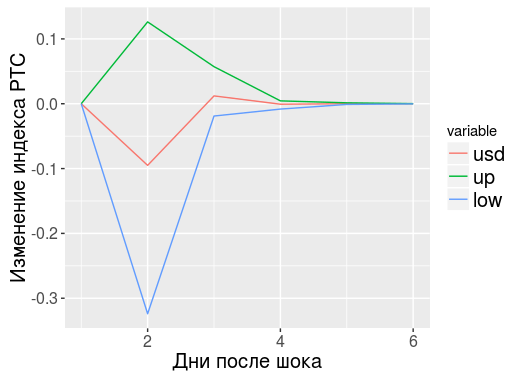
\includegraphics[width=1\linewidth]{Rplot_USD}}
\end{minipage}
\hfill
\begin{minipage}[H]{0.49\linewidth}
\center{\footnotesize{Индекс РТС} \\ 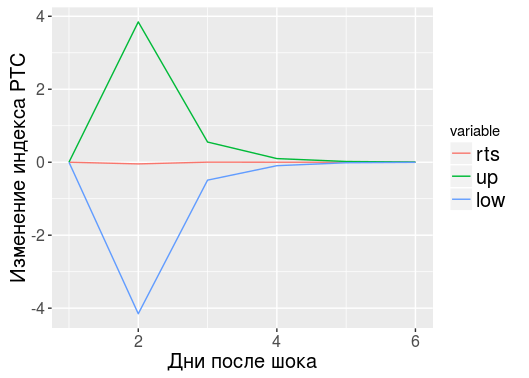
\includegraphics[width=1\linewidth]{Rplot_RTS}}
\end{minipage}
\vfill
\begin{minipage}[H]{0.49\linewidth}
\center{\footnotesize{Однодневная ставка МИАКР} \\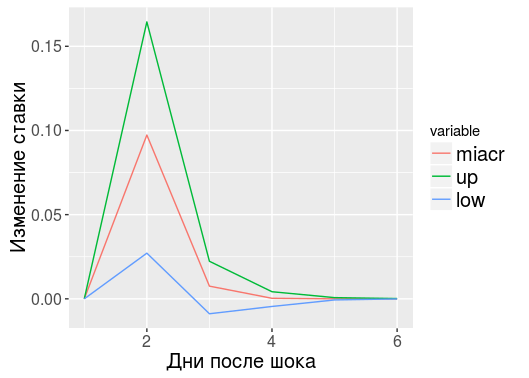
\includegraphics[width=1\linewidth]{Rplot_MIACR}}
\end{minipage}
\caption{Функции импульсного отклика валютного курса, индекса РТС и ставки МИАКР на заявления Банка России}
\label{otkl_1}
\end{figure}

При словесной интервенции Банка России происходит прыжок однодневной ставки МИАКР в течение следующего дня после заявления. В течение четырёх дней ставка МИАКР возвращается к своему прежнему уровню. Вторая спецификация подтверждает выводы, полученные при первой спецификации модели. Импульсные отклики валютного курса и индекса РТС на словесные интервенции Банка России оказываются снова незначимыми.



\chapter*{Заключение}
\addcontentsline{toc}{chapter}{Заключение}

Начиная с 2014 г. Банк России, в связи с переходом к режиму инфляционного таргетирования, начал иначе перестраивать свою информационную политику, повышая уровень предсказуемости и прозрачности. Управление ожиданиями постепенно налаживается, однако в Центробанке отмечают, что уровень репутации, необходимый для эффективного использования информационного канала, ещё не достигнут.

В данной работе были рассмотрены различные методы анализа влияния словесных интервенций на динамику различных макроэкономических переменных. С их помощью был проведён анализ информационной политики Банка России.





\nocite{*}  %Чтобы в список литературы напечаталичь все источники из bib-файла

% Если нам хочется, чтобы в списке литературы были не полуторные интервалы можно воспользоваться следующим приёмом: 
\begingroup
\setstretch{1}
\addcontentsline{toc}{chapter}{Список литературы}
\printbibliography[title = Список литературы]
\endgroup







%%%%%%%%%%%%%%%%%%%% Приложения %%%%%%%%%%%%%%%%%%%%

\appendix
\renewcommand{\thechapter}{\Asbuk{chapter}}

%%%%%%%%%% titlesec для приложений
\titleformat{\chapter}
 {\normalfont\bfseries\large}{\chaptertitlename~\thechapter}{0.25em}{\normalfont}


\titlecontents{chapter}
              [0 em] % 
              {\normalsize}
              {\makebox[7em][l]{Приложение \thecontentslabel}}
              {Приложение }
              {\titlerule*[10pt]{.}\contentspage}


\chapter[Программа~~  для~~ поиска~~ и~~ выгрузки~~   статей, касающихся Банка России из архива газеты Ведомости]{Программа для поиска и выгрузки статей, касающихся Банка Росии из архива газеты Ведомости (Python)}\label{app-a}

%\begin{minted}[breaklines]{python}
%def DaysOfYear(year):
%    def Days(month):
%        return([i for i in range(1,monthlength(month,2015)+1)])
%    s = []
%    for i in range(0,12):
%        s.append(Days(i))
%    return(s)
%
%cd "C:\Users\zero\Desktop\mydata"
%
%lll = DaysOfYear(2015)[0]
%for number in lll:
%    pickle.dump(getCBList(2015,1,number),
%    open(str(number)+'.txt', "wb" ))
%\end{minted}

Остальные месяцы выгружаются аналогичным образом. Теперь необходимо каждую из новостей, имеющих отношение к ЦБ дать оценку. Какой именно характер имеет словесная интервенция, отраженная в данной новости. Если она ведет к ужесточению политики, будем присваивать 1, если к смягчению, то -1. В итоге на выходе будем получать матрицу, каждая строка которой имеет вид [дата, смягчение или ужесточение].



\newpage
\thispagestyle{empty}

Выпускная квалификационная работа выполнена мной совершенно самостоятельно. Все использованные в работе материалы и концепции из опубликованной научной литературы и других источников имеют ссылки на них.

\vspace{2ex}

 Объем работы  \rule{2em}{0.5pt} листа(ов).

\vspace{2ex}

 Объем приложений \rule{2em}{0.5pt} листа(ов).

\vspace{4ex}

\noindent << \rule{1em}{0.5pt} >> \rule{5em}{0.5pt} 20 \rule{1.4em}{0.5pt} г. 

\vspace{4ex}

\noindent \rule{11em}{0.5pt} \hspace{8em} / Иванов Иван Иванович /

\end{document}
